\documentclass[12pt]{article}
\usepackage{amsfonts, amstext, amsmath, amsthm, amscd, amssymb, hyperref, float, longtable, fullpage}
\usepackage{epsfig, graphics, psfrag}
\usepackage{graphicx}
\usepackage{color}
\usepackage[font=small, labelfont=bf]{caption}
\usepackage{float}
\newtheorem{proposition}{Proposition}[section]
\newtheorem{theorem}{Theorem}[section]
\newtheorem{lemma}{Lemma}[section]
\newtheorem{corollary}{Corollary}[section]
\newtheorem{conjecture}{Conjecture}[section]
\newtheorem{claim}{Claim}[section]
\newtheorem{definition}{Definition}[section] 
\let\olddefinition\definition
\renewcommand{\definition}{\olddefinition\normalfont}
\newtheorem{remark}{Remark}[section]
\let\oldremark\remark
\renewcommand{\remark}{\oldremark\normalfont}
\newtheorem{question}{Question}[section]
\let\oldquestion\question
\renewcommand{\question}{\oldquestion\normalfont}
\newtheorem{notation}{Notation}[section]
\let\oldnotation\notation
\renewcommand{\notation}{\oldnotation\normalfont}
\newtheorem{example}{Example}[section]
\let\oldexample\example
\renewcommand{\example}{\oldexample\normalfont}
\newtheorem{algorithm}{Algorithm}[section]
\let\oldalgortihm\algorithm
\renewcommand{\algorithm}{\oldalgorithm\normalfont}
\newtheorem{method}{Method}[section]
\let\oldmethod\method
\renewcommand{\method}{\oldmethod\normalfont}
\let\oldemptyset\emptyset
\let\emptyset\varnothing
\newcommand{\ndiv}{\hspace{-4pt}\not|\hspace{2pt}}


\setlength{\parindent}{0in}

% DO NOT MAKE ANY CHANGES TO ANYTHING ABOVE THIS LINE. This is the ``preamble'' of the document that sets everything up. 

%%%%%%%%%%%%%%%%%%%%%%%%%%%%%%%%%%%%%%%%%%%%%%%%%%%%%%%%%%%%%%%%%%%%%%%%%%%%%%%%%%%%%%%%%%%%%%%%%%%%%%%%%%%%%%%%%%%%%%%



\title{{\bf{Math 3710W}} \\ Mathematical Modeling [Writing Portfolio]}

\author{Lixin Zheng}

\date{\today}

%%%%%%%%%%%%%%%%%%%%%%%%%%%%%%%%%%%%%%%%%%%%%%%%%%%%%%%%
%START BELOW %%%%%%%%%%%%%%%%

\begin{document}

\maketitle
\section{Linear Difference Equations}

\subsection{Introduction}

Linear difference equations are used to model biological processes mathematically. There are fundamental steps in mathematical modelling that necessitate the understanding and implementation of difference equations. The phases include developing the mathematical model that describes biological processes (formulation), applying mathematical techniques to explain model behaviour (analysis), and analysing the effects of the analysis (interpretation). Having said that, biological processes are represented using difference equations.
Difference equations are relationships between quantities as they vary over discrete time and space intervals. The difference equations are the differences between successive values of a function of a discrete variable are used to prove mathematical equality. 
We shall begin the study of difference equations by considering the first and simplest type of difference equation known as linear difference equations. The knowledge of linear difference equation can be fundamental. First, we give out some definitions of imperative terminologies and categorise different types of difference equations.Then we give some methods that could be used to solve linear difference equations. In the last section, we shall introduce and explain an example of linear difference equation referred to as Leslie matrix model. 
 

\subsection{Notations and Definitions}

Now let us consider about difference equation, the changes in states of a system are modelled over discrete intervals. The letter t is used to denote the time variable in most cases. The length of time interval is denoted as $\delta{t}$ in which the the discrete time models are t= 0, $\delta{t}$, 2$\delta{t}$ and so on. $\delta{t}$ =1 for easy definition of notation.
Suppose we denote the system at t as x(t). The lowercase letters denote the real variables while the capital letters denote the vectors of real variables. For instance, the notation Xt or X(t) is used when X is a vector. 


Let us give a precise definition of of first-order difference equation.

\begin{definition}
A difference equation of order k has the form 
\end{definition}

\begin{equation} 
f(x_{t+k}, x_{t+k-1}, …, x_{t+1}, x_{t}, t) =0 \tag{1.2.1}
\end{equation}

where f is dependent on $x_{t}$ and $x_{t+k}$ otherwise the order of the difference equation may be different from k. this is autonomous difference equation because f have nothing to do with t. otherwise it is called a non-autonomous equation.The assumption we will always lay in the difference equation is that the coefficients are real and the functions are real valued. 

The difference equation is usually used is in the form of:
\begin{equation}
x_{t+k}+a_{1}x_{t+k-1}+....+a_{k-1}x_{t+1}+a_{k}x_{1}=b_{t}\tag{1.2.2}
\end{equation}

The order of the difference equation (1.2.2) is k. The function $b_{t}$ may depend on t except the state variables.



\begin{definition}
The difference equation (1.2.2) is said to be linear if:
\end{definition}

the coefficients $a_{j},j=1,...k$ constant or depend on t but independent of the state variables. otherwise it is said to be non-linear.it is also said to be homogeneous if the difference equation (1.2.2) is linear and $b_{t}=0$. Otherwise, it is said to be non-homogeneous.  

\begin{definition}
If there is a k first-order difference equation, we can express it in the following form:
\begin{equation}
    x_{i}(t+1) = f_{i}(x_{1}(t), x_{2}(t),....x_{k}(t), t), i=1,2..k\tag{1.2.3}
\end{equation}
If the functions $f_{i}$ in the above equation is independent on t for i=1,2...k, we call it is autonomous.Otherwise, we can call it is non-autonomous.
\end{definition}


\begin{example}
Let us suppose such a difference equation: $x_{t+1} = ax_t^2+bx_{t-1}, a\neq0, b\neq0$. We call this equation is autonomous, second-order and non-linear.
\end{example}


\subsection{First-order difference equation}

a first-order, linear difference equation can be written in the form of:
\begin{equation}
    x_{t+1}=a_{t}x_{t}+b_{t}\tag{1.3.1}
\end{equation}
It is a typiacl difference equation. While the $b_t$ and $a_t$ is known, and $x_0$ is a Fixed value, there is some way to get a unique solution for it:

Let us consider about the $x_1$, that is :
\begin{equation}
    x_1 = a_0x_0 + b_0\tag{1.3.2}
\end{equation}
and it is the same for $x_{t+1} = a_tx_t + b_0$. Now we let $a_t = a$ and $b_t = b$, which can make the equation be simpler. This king of equation is called First order linear difference equation with constant coefficients. We can let the $t > 1$, in which way we can get a equation between $x{t+1}$ and $x_0$


\begin{equation}
    x_{t+1}=a^{t+1}x_{0}+b\sum_{i=0}^{t}c^{i}\tag{1.3.3}
\end{equation}
The above equation applies for constant coefficients $a_{t}=c$ and $b_{t}=b$.

one method that can be used to find the general solution when the coefficients are constant is demonstrated in the example below;

\begin{example}
let 
\begin{equation}
    x_{t+1}=ax_{t}+b\tag{1.3.4}
\end{equation}
where a and b are constants. The solution of (1.3.4) include a general solution and a particular solution.Since b is a constant, so we can get that the particular solution of this equation is a constant. We assume the solution is $x_p=k$, in which the k is a constant. In order to find the k, we can let the $x_{t+1}$ the same as $x_t$, then equation (1.3.5) can be got: 
\begin{equation}
    k=ak+b\tag{1.3.5}
\end{equation}
$k=b/(1-a)$ if a is not equal to 1. 
\end{example}
\setcounter{method}{0}
\begin{method}
To solve the problem of a first-order homogeneous equation, we do the following
\begin{enumerate}
    \item Step 1 Determine one particular solution of the non-homogeneous equation
    \item Step 2 Find the general solution of the homogeneous equation
    \item Step 3 The sum of step 1 and step 2 gives the general solution.
\end{enumerate}
\end{method}

\begin{example}Solve
\begin{equation}\label{DE}
    x_t = c + bx_{i+1}\tag{1.3.6}
\end{equation}
\end{example}

\noindent{\bf Solution.}
non-homogeneous equation is ct = c. we then look for a particular equation which could be $x_t = F$ as the constant. 
\begin{equation}
    F = c+bF\tag{1.3.7}
\end{equation}

The general solution is $x_t = Cb_t + c+b_F$

We have that

\begin{equation}
f(t, x_{t-1}) = bX_{t-1} + c\tag{1.3.8}
\end{equation}


We notice that c is a dependent variable while b is independent of t.\\
By method of successive calculation demonstrated in example 2.1, we could agree that the solution of the equation is:

\begin{equation*}
    x_t = b^t x_0 + \sum^t_{b^t-k} Ck\tag{1.3.9}
\end{equation*}
\\
\begin{example}
Now let us consider a practical problem which can be sloved by First-order difference equation:
Let us think about Pension issues, which we are all concerned. An old man deposits 200,000 dollars pension in the bank at the age of 60 with a monthly interest rate of $0.4\%$. Then He will take out 2,000 dollars a month as his living expenses, we can consider When will he run out of money:

This is a classical difference equation problem, so we can build a model by difference equation:
\begin{equation}
    A_{k+1} = aA_k - b\tag{1.3.10}
\end{equation}
where the $a = 1,04$ and $b = 2000$, and $A_0 = 200,000$. We can get the equation of $A_k$ that $A_n = a_nA_0 - b\frac{a_n - 1}{ra_n}$. For this difference equation, we need to let $A_n = 0$ and then $A_0 = \frac{b(a^n - 1)}{ra^n}$, where $r = 0.04$. We can use matlab to plot the figure:
\begin{figure}[htbp]
    \centering
    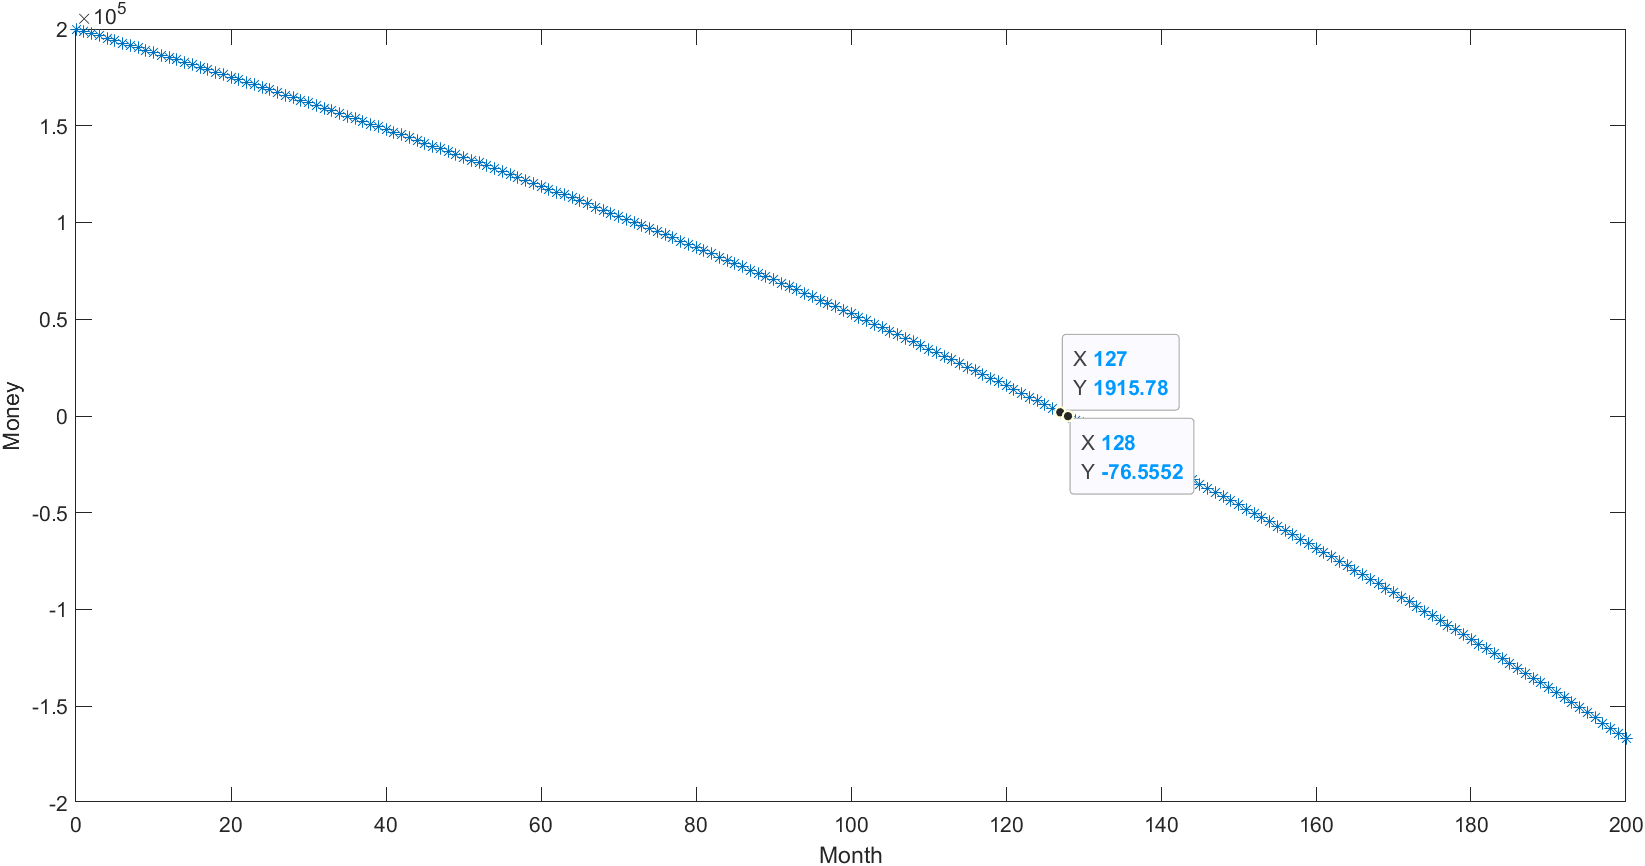
\includegraphics[scale=0.4]{difference_equation.png}
    \caption{The relationship between Time and Money}
    \label{fig:my_label}
\end{figure}
According to the figure, we can know that the old run out of his money when the Month is 128.
\end{example}

\subsection{Second-Order and Higher-Order Equations}
For Higher-Order Equations, there is a new method to slove the kth-order, non-homogeneous, linear difference equation. Let us consider the general solution, it is a function of k constants, which is uniquely decided by $x_0, x_1...$. It can also be used in homogeneous, second-order, linear difference equation with constant coefficients\\\\

If we have the difference equation,
\begin{equation}
    x_{t+2}+ax_{t+1}+bx_{t}=0\tag{1.4.1}
\end{equation}
given that a and b are constants. assume the solution has $x_{t}=\lambda^{t}$. Then we can get:
\begin{equation*}
    \lambda^{t+2}+a\lambda^{t+1}+b\lambda^{t}=0\tag{1.4.2}
\end{equation*}
\begin{equation*}
    \lambda^{t}(\lambda^{2}+a\lambda+b)=0\tag{1.4.3}
\end{equation*}

\begin{definition}
The equation $\lambda^2+a\lambda+b=0$ is called the characteristic equation and $\lambda^{2}+a\lambda+b$ is called the characteristic polynomial of the difference equation(2.4.1).\\\\
For equation (1.4.1) to be second order, b is not equal to 0. Therefore, none of the eigenvalues of the characteristic equation can be zero.\\\\
\end{definition}

\subsubsection{Case 1}
If the eigenvalues are real and distinct,$\lambda_1$ is not equal to $\lambda_2$.then the two linearly independent solutions are $x^{1}=\lambda_1$ and $x^2=\lambda^{t}_2$. The general solution is \\\\
\begin{equation}
    x_t=c_1\lambda^{t}_1+c_2\lambda^{t}_2\tag{1.4.1.1}
\end{equation}

\subsubsection{Case 2}
Suppose the eigenvalues are real and equal, $\lambda_1=\lambda_2$. Then the two linearly independent solutions are $x^1=\lambda^t_{1}$ and $x^2=t\lambda^t_{1}$. The general solution is\\\\
\begin{equation}
    x_t=c_1\lambda^t_{1}+c_2t\lambda^t_{1}\tag{1.4.1.2}
\end{equation}

The solutions $x^1$ and $x^2$ are linearly independent.

\begin{example}
Consider this third-order, homogeneous equation
\begin{equation*}
    x_{t+3}+x_{t+2}+x_{t+1}+x{t}=0\tag{1.4.1.3}
\end{equation*}

The equation satisfies $\lambda^3+\lambda^2+\lambda+1=0$ \\\\
This can also be factorised and written as $(\lambda+1)(\lambda^2+1)=0$\\\\
The general solution to the homogeneous equation is given by
\begin{equation*}
    x_t=c_1(-1)^1+c_2cos(t\pi/2)-c_3sin(t\pi/2)\tag{1.4.1.4}
\end{equation*}
The difference equation is non-homogeneous if
\begin{equation*}
    x_{t-3}+x_{t+2}+x_{t+1}+x_{t}=4t\tag{1.4.1.5}
\end{equation*}
we need to find the non-homogeneous equation in order to find the general solution. we assume the particular solution is a linear polynomial in t:\\\\
\begin{equation*}
    x_p=k_1t+k_2\tag{1.4.1.6}
\end{equation*}
Then we substitute the value of $x_p$ into the non-homogeneous difference equation\\\\
\begin{equation*}
    k_1(t+3)+k_2+k_1(t+2)+k_2+k_1(t+1)+k_2+k_1t+k_2=4t\tag{1.4.1.7}
\end{equation*}
when we simplify, we get;
\begin{equation*}
    4k_1t+6k_1+4k_2=4t\tag{1.4.1.8}
\end{equation*}
The coefficients are equated such that $4k_1=4$ and $6k_1+4k_2=0$. the values of k1 and k2 are $k_1=1$ and $k_2=-3/2$.The general solution is:
\begin{equation*}
    x_t=x_h+x_p=c_1(-1)^1+c_2cos(t\pi/2)+c_3sin(t\pi/2)+t-3/2\tag{1.4.1.9}
\end{equation*}

\end{example}
\subsection{Logistic Model}
Logistic Model is a classical ecological model, which is proposed famous ecologist Robert May. The difference equation of Logistic Model is as following:
\begin{equation}
    x_{k+1} = bx_k(1-x_k)\tag{1.5.1}
\end{equation}
First of all, we can let $x_{k+1} = x_k$ to calculate the balance point, which is $x_1^* = 0$ and $x_2^* = 1 - \frac{1}{b}$. There are three cases for it:

case1 : If $b < 1$, there is only one balance point $x_1^*$;

case2 : If $1 < b < 3$, $x_2^*$ will be the only one balance point;

case3 : If $b > 3$, there is no balance point;

Now there is a ecological example which is modelling with Logistic Model. There are two species in the same region. In the absence of other populations, each population can grow infinitely. The existence of the second population will reduce the growth rate of the first population, which is is proportional to the product of the number of the two species.

Then, we can build a model as following:
\begin{equation}
    \Delta x_n = k_1x_n - k_3x_ny_n\tag{1.5.2}
\end{equation}
\begin{equation}
    \Delta y_n = k_2y_n - k_4x_ny_n\tag{1.5.3}
\end{equation}
we assume $k_1 = 0.2, k_2 = 0.3, k_3 = 0.001, k_4 = 0.004$, then:
\begin{equation}
    \begin{cases}
    x_{n+1} = 1.2x_n - 0.001x_n y_n \\
    y_{n+1} = 1.3y_n - 0.002x_n y_n \\
    \end{cases}\tag{1.5.4}
\end{equation}
The balance point is (0, 0) and (150, 200), Then let us consider three case:

\subsubsection{case1}
    When the $x_0 = 151$ and $y_0 = 199$, which represents the initial number of two species. We can know in the figure how the number of them change:
    \begin{figure}[htbp]
    \centering
    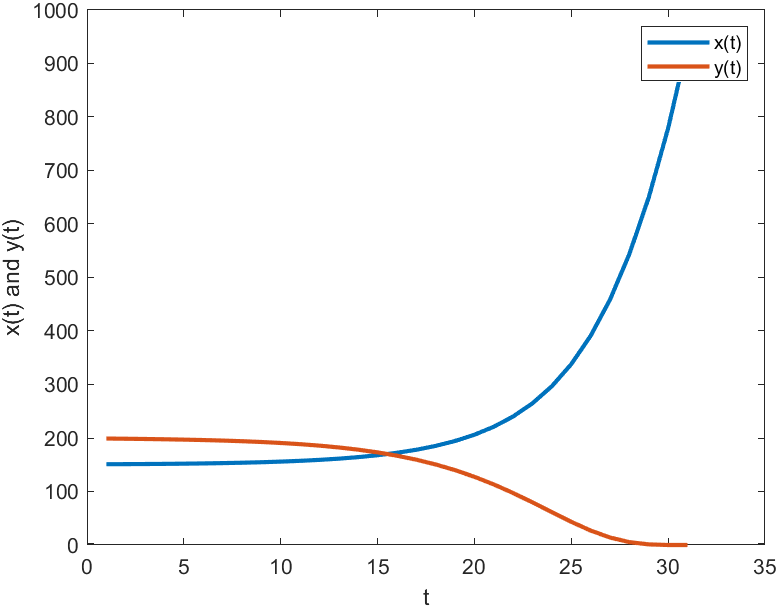
\includegraphics[scale=0.5]{numbers_1.png}
    \caption{the changes when x0 = 151 and y0 = 199}
    \label{fig:my_label}
\end{figure}
In this case, we can see that the $x_t$ become more and more and $y_t$ become less and less.
\subsubsection{case2}
This case we consider that if $x_0 = 149$ and $y_0 = 201$, the figure is as following:
    \begin{figure}[H]
    \centering
    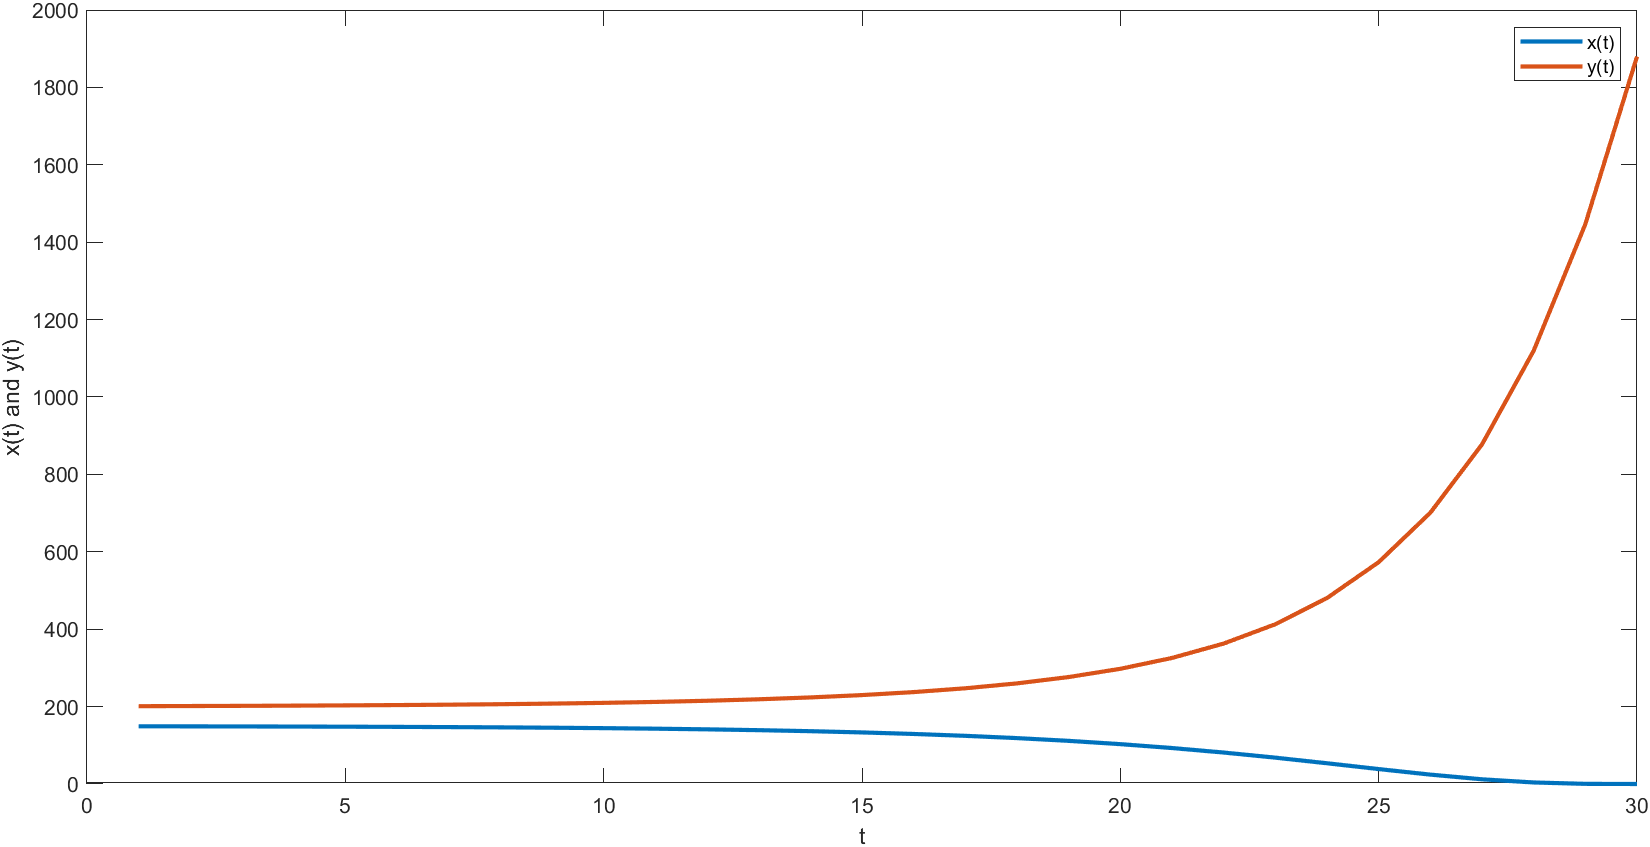
\includegraphics[scale=0.3]{numbers_2.png}
    \caption{the changes when x0 = 151 and y0 = 199}
    \label{fig:my_label}
\end{figure}
On the contract, the $x_t$ become less and less and $y_t$ become more and more.
\subsubsection{case3}
In this case, we will let $x_0 = 10$ and $y_0 = 10$. The same wat, let us look at the figure at first:
    \begin{figure}[H]
    \centering
    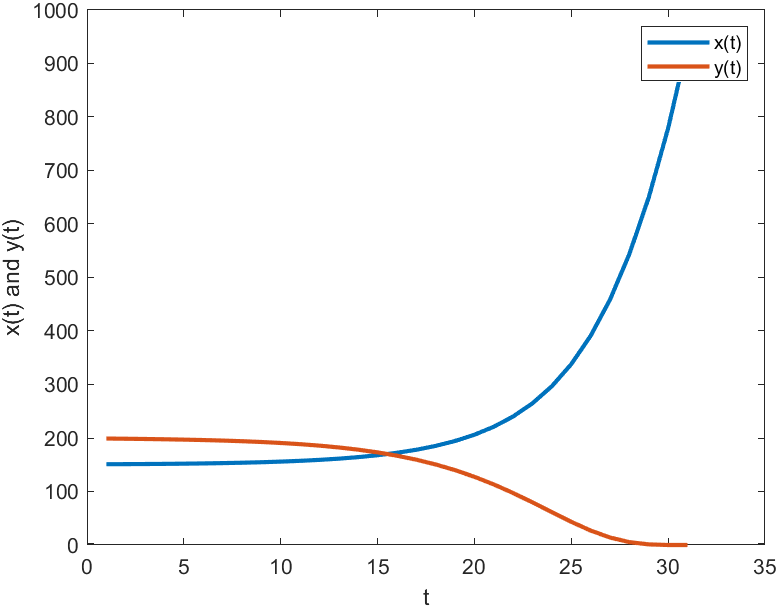
\includegraphics[scale=0.5]{numbers_1.png}
    \caption{the changes when x0 = 10 and y0 = 10}
    \label{fig:my_label}
\end{figure}
Now there is a interesting phenomenon. At first, the $x_t$ will increase and $y_t$ increase, too. After increasing for about 16 times, $x_t$ will decrease but $y_t$ increase faster.

Like the example 1.4, the code will be given on the last.
\subsection{Summary}

We have discussed and seen how to work with difference equations. The derivation of general solutions for non-homogeneous and homogeneous solutions has been discussed. The knowledge of difference equation is fundamental in non-linear difference equation, and therefore this part of the whole problem of discussion is very important to master and understand. The reader should not confuse the two terms and how they should be used in solving mathematical problems. 
\subsection{Codes}
Example 1.4:

x0 = 200000; n = 200;

b = 2000; r = 0.004

k = (0:n)';

y1 = dai(x0, n, r, b)

round([k, y1'])

plot(k, y1', '*')

xlabel('Month')

ylabel('Money')

p = 128;

text(x(p),y(p),['(',num2str(x(p)),',',num2str(y(p)),')'],'color','b')

function x = dai(x0, n, r, b)

a = 1+r;

x = x0;

for k = 1:n

    x(k+1) = a*x(k)-b;

end

end

Logistic Mode:
k1 = 1.2;

k2 = 1.3;

k3 = 0.001;

k4 = 0.002;

x(1) = 10;

y(1) = 10;

for k = 1:1:25

    x(k+1) = k1*x(k) - k3*x(k)*y(k);

    y(k+1) = k2*y(k) - k4*x(k)*y(k);

end

figure;

t = 1:1:26;

plot(t,x,'LineWidth',2);

hold on;

plot(t,y,'LineWidth',2);

legend('x(t)','y(t)');

ylabel('x(t) and y(t)');

xlabel('t');



\begin{thebibliography}{4}
\bibitem{came}
https://en.wikipedia.org/wiki/Applied\_mathematics
\bibitem{came}
https://www.nature.com/subjects/applied-mathematics
\bibitem{came}
https://www.siam.org/Portals/0/Student\%20Programs/Thinking\%20of\%20a\%20Ca
reer/brochure.pdf
\bibitem{came}
https://en.wikipedia.org/wiki/Coronavirus\_disease\_2019
\bibitem{came}
LindaJ.S.Allen-AnIntroductiontoMathematicalBiology-Pearson(2006)
\end{thebibliography}
\end{document}